
%-----------------
% Back page

\newcommand*\cleartoleftpage{%
  \clearpage
  \ifodd\value{page}\hbox{}\newpage\fi
}

\cleartoleftpage

\backgroundsetup{%
    scale=1.7,
    angle=0,
    contents={%
        \begin{tikzpicture}
            %\pgfmathsetmacro{\myopacity}{mod(\thepage-1,4)*0.25+0.25}
            \node[opacity=0.35] {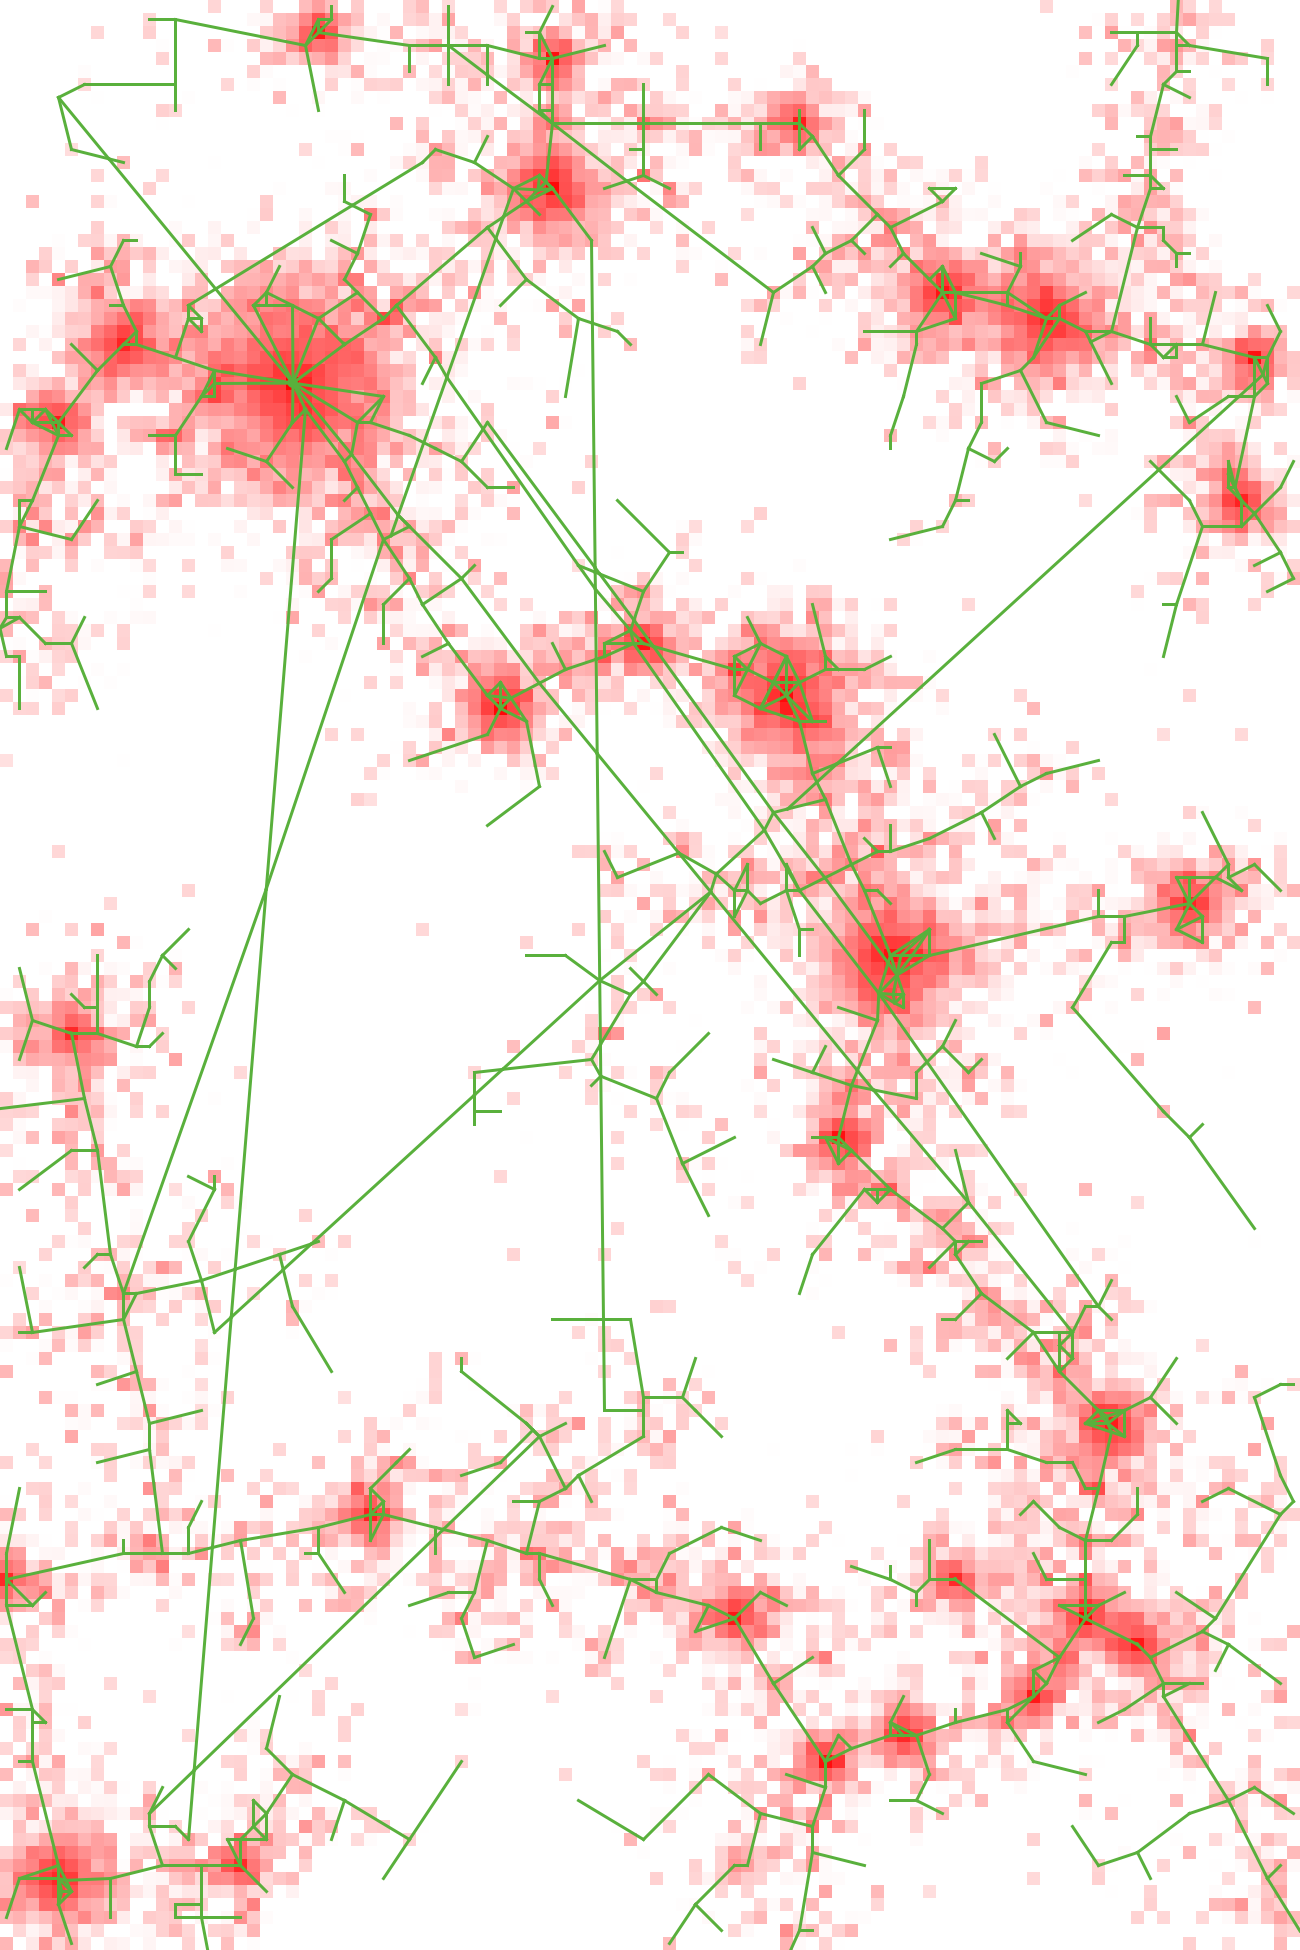
\includegraphics[width=\linewidth]{Figures/Cover/cover2}};
        \end{tikzpicture}
    }
}

\markboth{}{}

%\newgeometry{margin=2cm}
\pagenumbering{gobble}

\begin{adjustwidth*}{-1.8cm}{-4.0cm}

\small

\bpar{
\noindent\textbf{Characterizing and modeling the co-evolution of transportation networks and territories}
}{
\noindent\textbf{Caractérisation et modélisation de la co-évolution des réseaux de transport et des territoires}
}

\bigskip

\bpar{
\noindent\textbf{Keywords: } Territories; Transportation Networks; Co-evolution; Morphogenesis; Evolutive Urban Theory; Quantitative Epistemology; Systems of Cities; Urban Morphology; Greater Paris; Pearl River Delta
}{
\noindent\textbf{Mots-clés : } Territoires ; Réseaux de Transport ; Co-évolution ; Morphogenèse ; Théorie Évolutive des Villes ; Épistémologie Quantitative ; Systèmes de Villes ; Morphologie Urbaine ; Grand Paris ; Delta de la Rivière des Perles
}

\bigskip

\bpar{
\noindent
The identification of structuring effects of transportation infrastructure on territorial dynamics remains an open research problem. This issue is one of the aspects of approaches on complexity of territorial dynamics, within which territories and networks would be co-evolving. The aim of this thesis is to challenge this view on interactions between networks and territories, both at the conceptual and empirical level, by integrating them in simulation models of territorial systems. The intrinsically multidisciplinary nature of the question requires first to proceed to a quantitative epistemology analysis, that allow us to draw a map of the scientific landscape and to give a description of common features and specificities of models studying the co-evolution between network and territories within each discipline. We propose consequently a definition of co-evolution and an empirical method for its characterization, based on spatio-temporal correlation analysis. Two complementary modeling approaches, that correspond to different scales and ontologies, are then explored. At the macroscopic scale, we build a family of models inheriting from interaction models within system of cities, developed by the Evolutive Urban Theory (Pumain, 1997). Their exploration shows that they effectively capture co-evolutionary dynamics, and their calibration on demographic data for the French system of cities (1830-1999) quantifies the evolution of interaction processes such as the tunnel effect or the role of centrality. At the mesoscopic scale, a morphogenesis model captures the co-evolution of the urban form and of network topology. It is calibrated on corresponding indicators for local form and topology, computed for all Europe. Multiple network evolution processes are shown complementary to reproduce the large variety of observed configurations, at the level of indicators but also interactions between indicators. These results suggest new research directions for urban models integrating co-evolutive dynamics in a multi-scale perspective.
}{
\noindent
L'identification d'effets structurants des infrastructures de transports sur la dynamique des territoires reste un défi scientifique ouvert. Cette question est une des facettes de recherches sur la complexité des dynamiques territoriales, au sein desquelles territoires et réseaux de transport seraient en co-évolution. L'objectif de cette thèse est de mettre à l'épreuve cette vision des interactions entre réseaux et territoires, autant sur le plan conceptuel que sur le plan empirique, en les intégrant au sein de modèles de simulation des systèmes territoriaux. La nature intrinsèquement pluri-disciplinaire de la question nous conduit à mener un travail d'épistémologie quantitative, qui permet de dresser une carte du paysage scientifique et une description des éléments communs et des spécificités des modèles traitant la co-évolution entre réseaux et territoires dans chaque discipline. Nous proposons ensuite une définition de la co-évolution, ainsi qu'une méthode de caractérisation empirique, basée sur une analyse de corrélations spatio-temporelles. Deux pistes complémentaires de modélisation, correspondant à des ontologies et des échelles différentes sont alors explorées. A l'échelle macroscopique, nous construisons une famille de modèles dans la lignée des modèles d'interaction au sein des systèmes de villes développés par la Théorie Evolutive des Villes (Pumain, 1997). Leur exploration montre qu'ils capturent effectivement des dynamiques de co-évolution, et leur calibration sur des données démographiques pour le système de villes français (1830-1999) quantifie l'évolution des processus d'interaction comme l'effet tunnel ou le rôle de la centralité. A l'échelle mésoscopique, un modèle de morphogenèse capture la co-évolution de la forme urbaine et de la topologie du réseau. Il est calibré sur les indicateurs correspondants pour la forme et la topologie locales calculés pour l'ensemble de l'Europe. De multiples processus d'évolution du réseau s'avèrent être complémentaires pour reproduire la grande variété des configurations observées, au niveau des indicateurs ainsi que des interactions entre indicateurs. Ces résultats suggèrent de nouvelles pistes d'exploration des modèles urbains intégrant les dynamiques co-évolutives dans une perspective multi-échelles.
}

\vspace{1.3cm}

\bpar{
\noindent\textbf{Caractérisation et modélisation de la co-évolution des réseaux de transport et des territoires}
}{
\noindent\textbf{Characterizing and modeling the co-evolution of transportation networks and territories}
}

\bigskip

\bpar{
\noindent\textbf{Mots-clés : } Territoires ; Réseaux de Transport ; Co-évolution ; Morphogenèse ; Théorie Évolutive des Villes ; Épistémologie Quantitative ; Systèmes de Villes ; Morphologie Urbaine ; Grand Paris ; Delta de la Rivière des Perles
}{
\noindent\textbf{Keywords: } Territories; Transportation Networks; Co-evolution; Morphogenesis; Evolutive Urban Theory; Quantitative Epistemology; Systems of Cities; Urban Morphology; Greater Paris; Pearl River Delta
}

\bigskip

\bpar{
\noindent
L'identification d'effets structurants des infrastructures de transports sur la dynamique des territoires reste un défi scientifique ouvert. Cette question est une des facettes de recherches sur la complexité des dynamiques territoriales, au sein desquelles territoires et réseaux de transport seraient en co-évolution. L'objectif de cette thèse est de mettre à l'épreuve cette vision des interactions entre réseaux et territoires, autant sur le plan conceptuel que sur le plan empirique, en les intégrant au sein de modèles de simulation des systèmes territoriaux. La nature intrinsèquement pluri-disciplinaire de la question nous conduit à mener un travail d'épistémologie quantitative, qui permet de dresser une carte du paysage scientifique et une description des éléments communs et des spécificités des modèles traitant la co-évolution entre réseaux et territoires dans chaque discipline. Nous proposons ensuite une définition de la co-évolution, ainsi qu'une méthode de caractérisation empirique, basée sur une analyse de corrélations spatio-temporelles. Deux pistes complémentaires de modélisation, correspondant à des ontologies et des échelles différentes sont alors explorées. A l'échelle macroscopique, nous construisons une famille de modèles dans la lignée des modèles d'interaction au sein des systèmes de villes développés par la Théorie Evolutive des Villes (Pumain, 1997). Leur exploration montre qu'ils capturent effectivement des dynamiques de co-évolution, et leur calibration sur des données démographiques pour le système de villes français (1830-1999) quantifie l'évolution des processus d'interaction comme l'effet tunnel ou le rôle de la centralité. A l'échelle mésoscopique, un modèle de morphogenèse capture la co-évolution de la forme urbaine et de la topologie du réseau. Il est calibré sur les indicateurs correspondants pour la forme et la topologie locales calculés pour l'ensemble de l'Europe. De multiples processus d'évolution du réseau s'avèrent être complémentaires pour reproduire la grande variété des configurations observées, au niveau des indicateurs ainsi que des interactions entre indicateurs. Ces résultats suggèrent de nouvelles pistes d'exploration des modèles urbains intégrant les dynamiques co-évolutives dans une perspective multi-échelles.
}{
\noindent
The identification of structuring effects of transportation infrastructure on territorial dynamics remains an open research problem. This issue is one of the aspects of approaches on complexity of territorial dynamics, within which territories and networks would be co-evolving. The aim of this thesis is to challenge this view on interactions between networks and territories, both at the conceptual and empirical level, by integrating them in simulation models of territorial systems. The intrinsically multidisciplinary nature of the question requires first to proceed to a quantitative epistemology analysis, that allow us to draw a map of the scientific landscape and to give a description of common features and specificities of models studying the co-evolution between network and territories within each discipline. We propose consequently a definition of co-evolution and an empirical method for its characterization, based on spatio-temporal correlation analysis. Two complementary modeling approaches, that correspond to different scales and ontologies, are then explored. At the macroscopic scale, we build a family of models inheriting from interaction models within system of cities, developed by the Evolutive Urban Theory (Pumain, 1997). Their exploration shows that they effectively capture co-evolutionary dynamics, and their calibration on demographic data for the French system of cities (1830-1999) quantifies the evolution of interaction processes such as the tunnel effect or the role of centrality. At the mesoscopic scale, a morphogenesis model captures the co-evolution of the urban form and of network topology. It is calibrated on corresponding indicators for local form and topology, computed for all Europe. Multiple network evolution processes are shown complementary to reproduce the large variety of observed configurations, at the level of indicators but also interactions between indicators. These results suggest new research directions for urban models integrating co-evolutive dynamics in a multi-scale perspective.
}


\end{adjustwidth*}



